% Appendix C
 
\chapter{Additional Plots \& Tables}
\label{sec:appendiximages}

This appendix provides additional charts that can be helpfull fore more in depth understanding

\section{Dataset Analysis}\label{AppendixDatasetAnalysis}

\begin{figure*}[htb]
    \centering
    \begin{minipage}{1.5\textwidth}
        \centering
        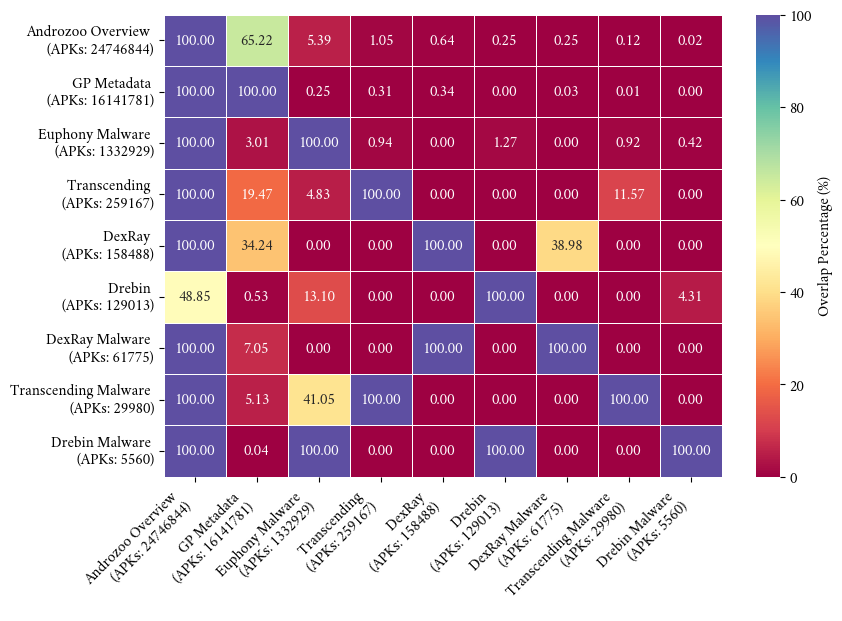
\includegraphics[width=\textwidth]{A_Images/heatmap_sha256_overlaps_percentage.png}
        \captionsetup{width=\textwidth}
        \caption{\label{fig:dataset_overlap}
        Overlap percentages among various Android malware datasets and Google Play metadata provided by \cite{gp_metadata}. 
        The diagonal values represent 100\% overlap (self-comparison), 
        while off-diagonal values highlight shared entries between datasets.
        Notable is that DexRay-, Transcending-, and Drebin Malware are subsets of Androzoo,
        but only partially of Androzoo malware.
        }
    \end{minipage}
\end{figure*}

\newpage

\begin{figure*}[h]
    \centering
    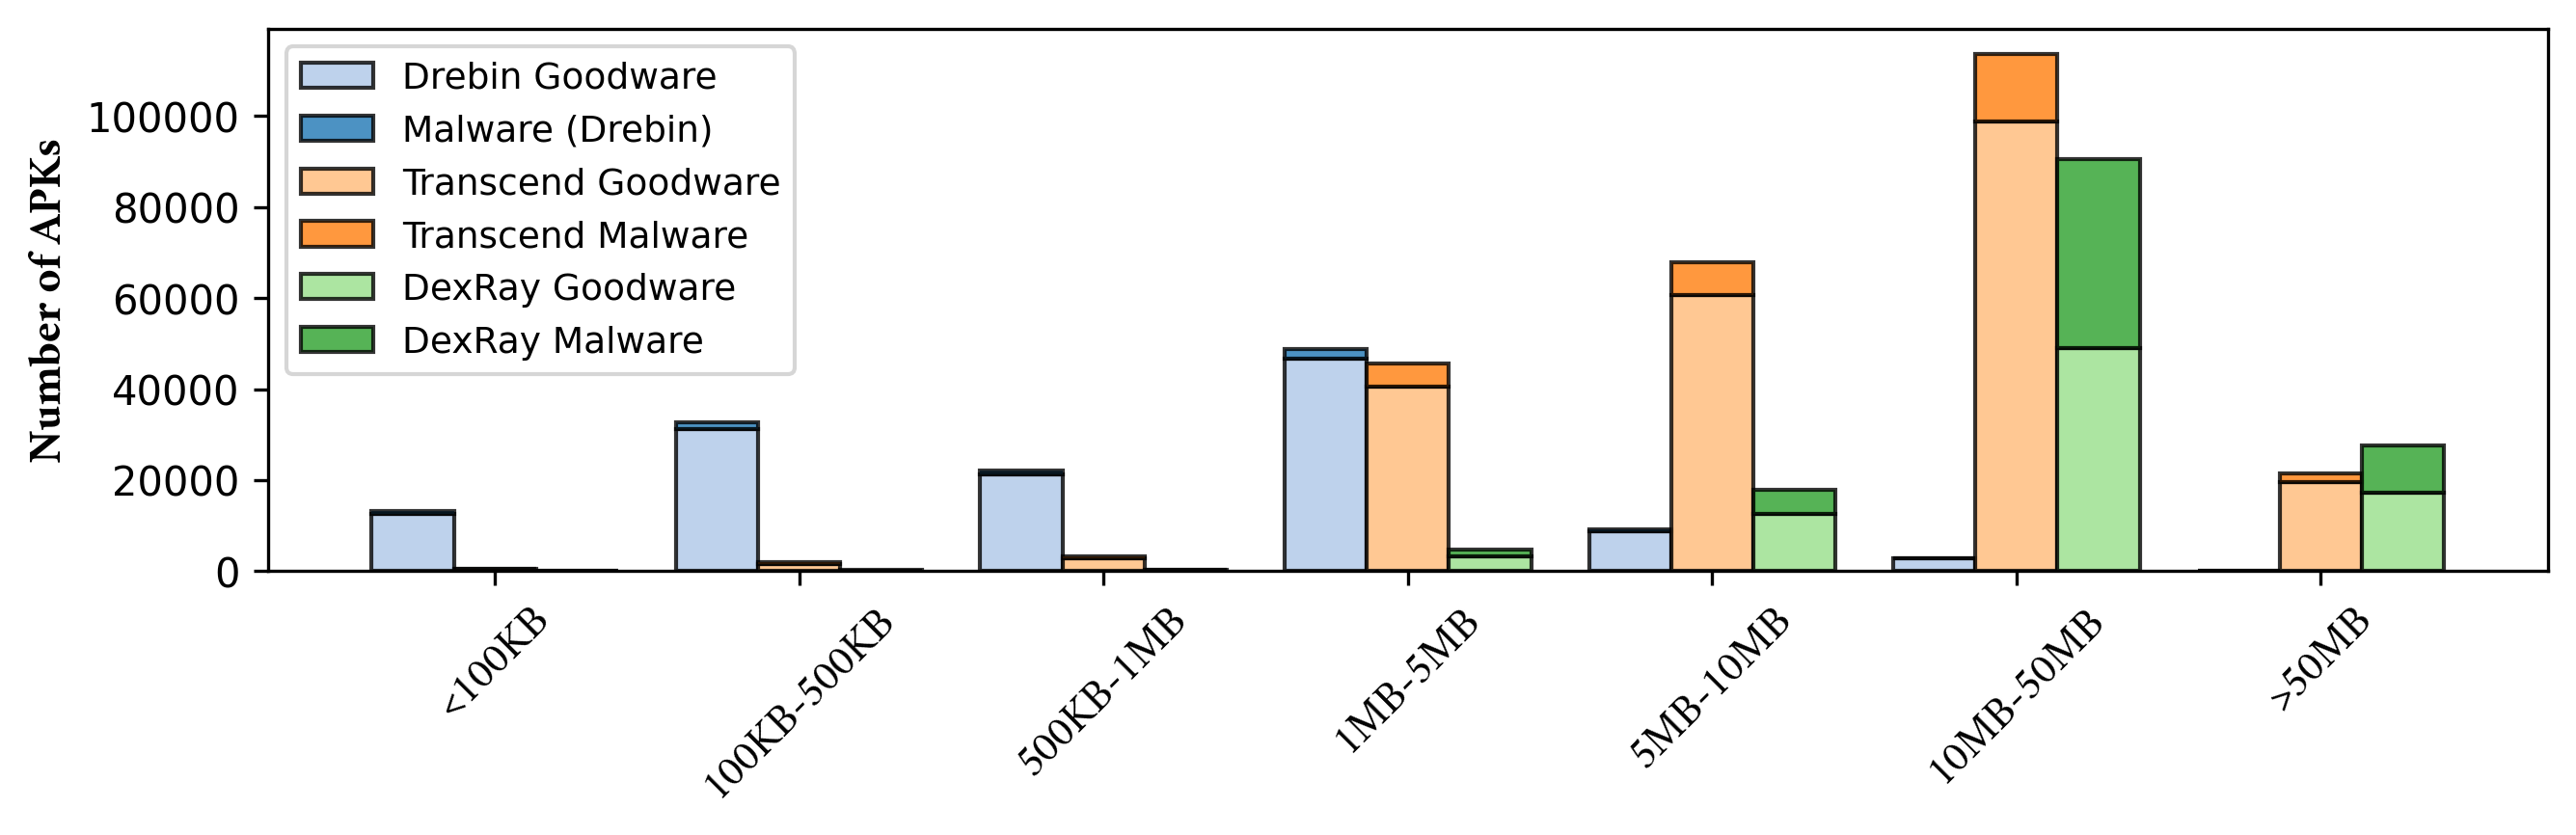
\includegraphics[width=\widefigurewidth]{3_Methodology/dataset_size_distribution.png}
    \caption{\label{fig:dataset_size_evaluation}
    Temporal distribution of Android APKs across three datasets (Drebin, Transcend, and DexRay), 
    categorized into goodware and malware.}
\end{figure*}



\begin{figure*}[b!]
    \centering
    \begin{minipage}{1.5\textwidth}
        \centering
        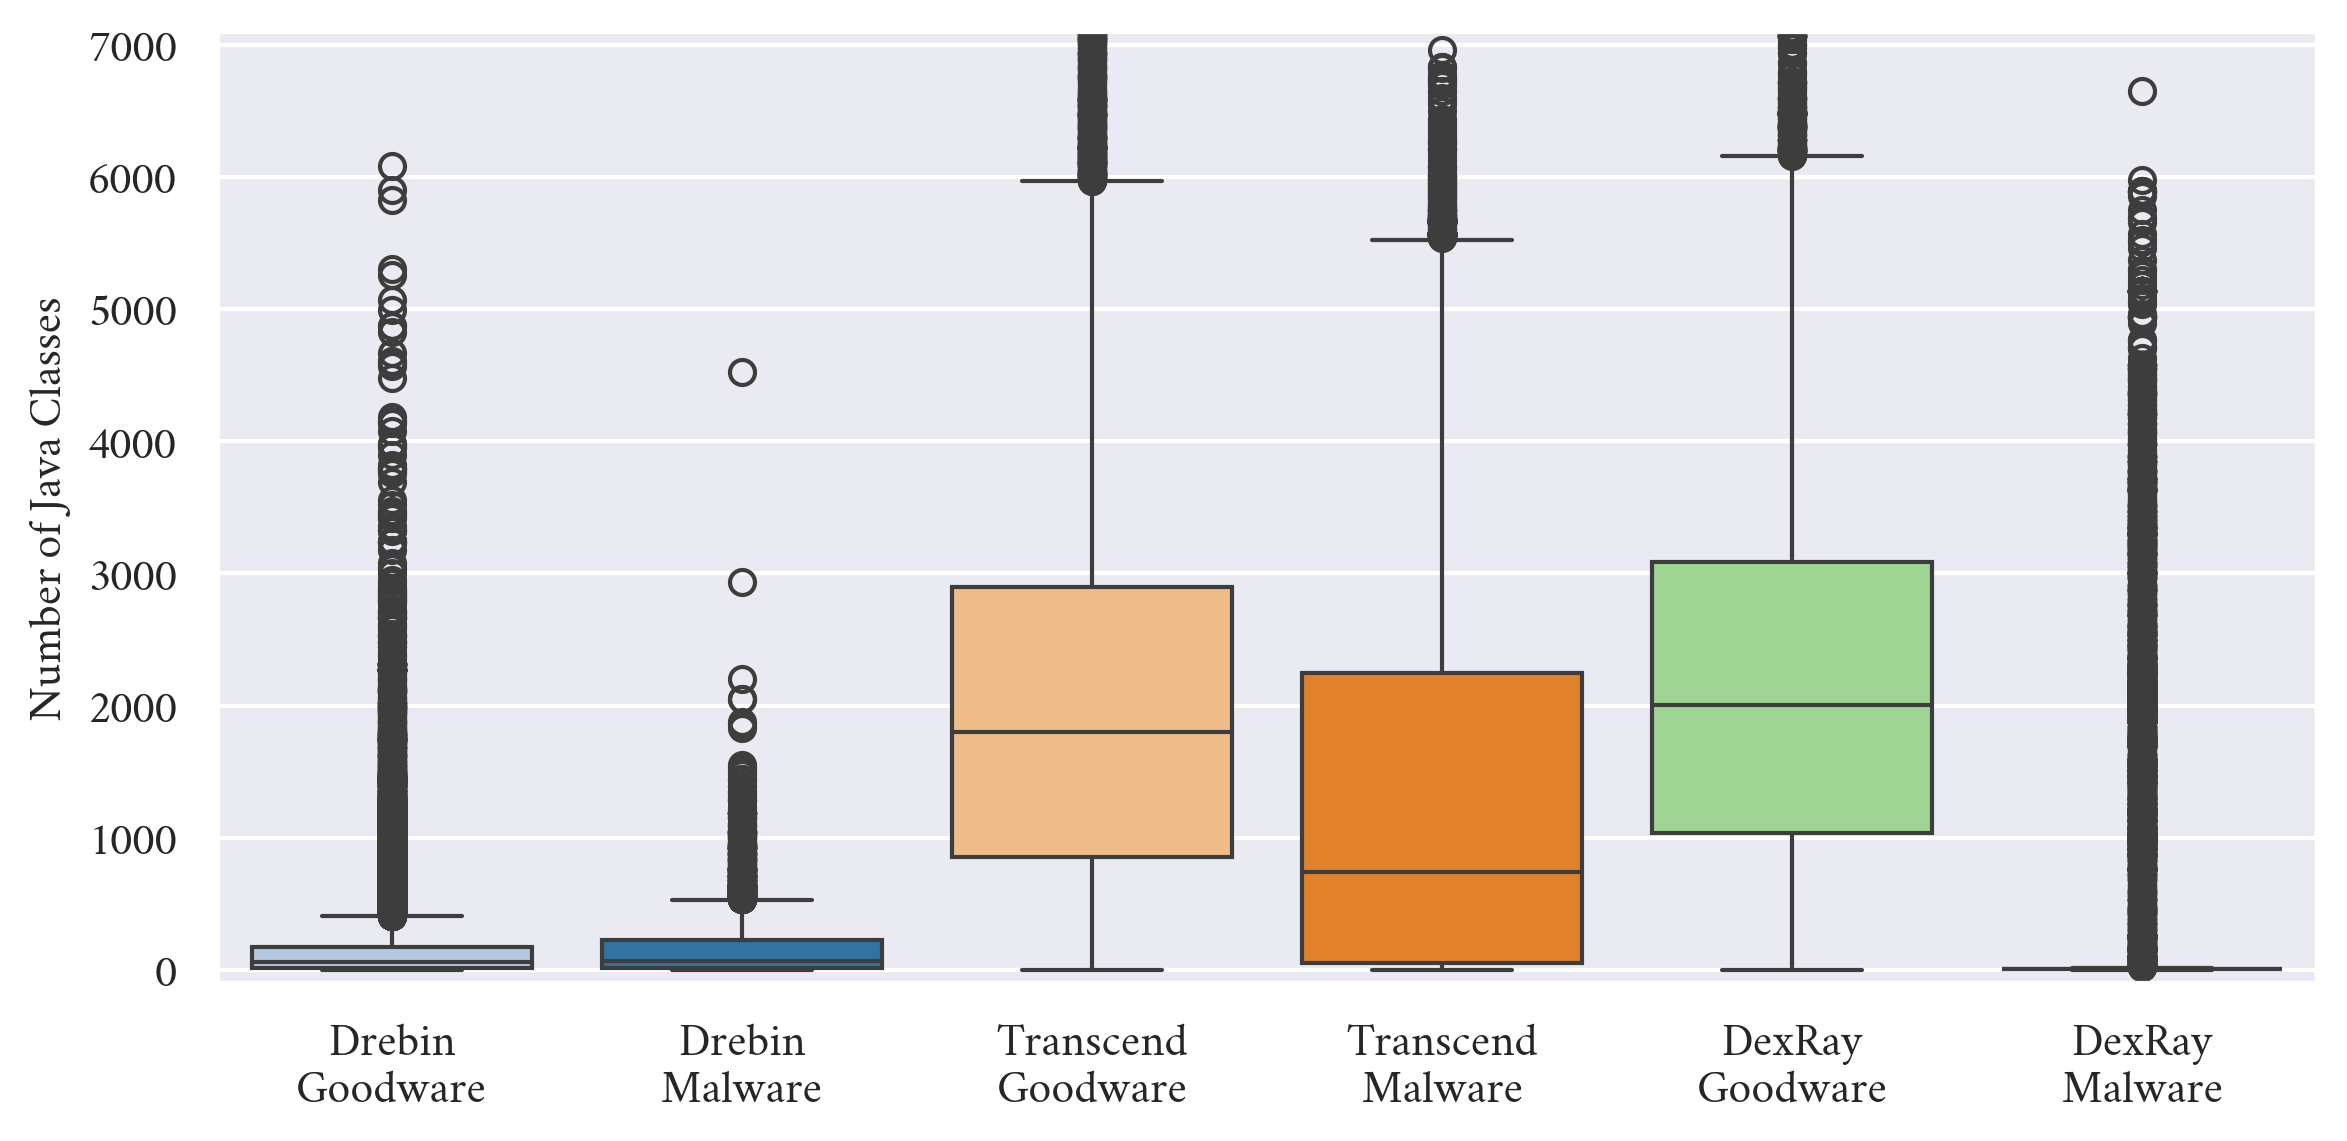
\includegraphics[width=\textwidth]{3_Methodology/java_class_boxplots.png}
        \captionsetup{width=\textwidth}
        \caption{\label{fig:java_class_boxplots}
        The boxplot shows the distribution of Java classes in Android apps 
        across the Drebin, Transcend, and DexRay datasets, 
        split into Goodware and Malware. 
        Drebin and Transcend have an similar java class distribution 
        between Goodware and Malware.
        The DexRay Dataset shows a high inbalance in the number of java classes 
        between the two labels.
        }
    \end{minipage}
\end{figure*}

\newpage

\section{Baseline Creation}\label{AppendixBaselineCreation}

\vspace{0em} % Adjust vertical spacing after the section header if needed

\begin{table}[h!]
    \caption{\label{tab:decisiontree}%
    Decision Tree (max\_depth=15) results by dataset and split. Features include Java Classes, Smali Classes, and APK Size.}
    \centering
    \small % Reduce font size for the table
    \begin{tabular}{@{}llcccc@{}}
    \toprule
    \textbf{Dataset} & \textbf{Split} & \textbf{Accuracy} & \textbf{Precision} & \textbf{Recall} & \textbf{F1 Score} \\ \cmidrule(r){1-2} \cmidrule(lr){3-6}
    Drebin         & random     & 90.98\% & 28.13\% & 74.56\% & 40.84\% \\
                   & time based & 80.94\% & 8.99\%  & 37.50\% & 14.50\% \\ \addlinespace
    Transcending   & random     & 88.34\% & 49.57\% & 70.86\% & 58.33\% \\
                   & time based & 85.36\% & 40.46\% & 56.30\% & 47.09\% \\ \addlinespace
    DexRay         & random     & 96.20\% & 96.56\% & 93.74\% & 95.13\% \\
                   & time based & 92.82\% & 85.35\% & 98.30\% & 91.37\% \\
    \bottomrule
    \end{tabular}
\end{table}

\vspace{2em} % Adjust vertical spacing between tables

\begin{table}[h!]
    \caption{\label{tab:decisiontreecombined}%
    Decision Tree (max\_depth=15) results by dataset and split. Features include Java Classes, Smali Classes, APK Size, and Permissions.}
    \centering
    \small % Reduce font size for the table
    \begin{tabular}{@{}llcccc@{}}
    \toprule
    \textbf{Dataset} & \textbf{Split} & \textbf{Accuracy} & \textbf{Precision} & \textbf{Recall} & \textbf{F1 Score} \\ \cmidrule(r){1-2} \cmidrule(lr){3-6}
    Drebin         & random     & 97.10\% & 60.59\% & 89.35\% & 72.21\% \\
                    & time based & 90.66\% & 30.55\% & 91.55\% & 45.81\% \\ \addlinespace
    Transcending   & random     & 92.55\% & 62.81\% & 87.03\% & 72.96\% \\
                    & time based & 91.15\% & 59.08\% & 76.14\% & 66.53\% \\ \addlinespace
    DexRay         & random     & 96.87\% & 96.82\% & 95.21\% & 96.01\% \\
                    & time based & 96.10\% & 91.74\% & 98.82\% & 95.15\% \\
    \bottomrule
    \end{tabular}
\end{table}

\newpage

\section{Evalutaion}\label{AppendixEvalutaion}

\vspace{0em} % Adjust vertical spacing after the section header if needed


\begin{table}[h] 
    \caption{\label{tab:encoder_model_comparison_average}%
    Performance comparison of different encoder models for generating embeddings. The APK representation is fixed to Activities (A) and Permissions (P). The encoder was trained through backpropagation in this experiment. The transcenden subset was used as dataset. The average of all tokens was used to calculate a single embedding as APK representation.}    
    \resizebox{\textwidth}{!}{%
    \begin{tabular}{@{}lcccc@{}}
    \toprule
    \textbf{Model} & \textbf{Accuracy} & \textbf{Precision} & \textbf{Recall} & \textbf{F1} \\ 
    \cmidrule(r){1-1} \cmidrule(lr){2-5}
    modernBERT & 82.38\% & 86.29\% & 76.81\% & 81.28\% \\
    BigBird    & 63.10\% & 64.27\% & 58.28\% & 61.13\% \\
    Longformer & 62.50\% & 62.93\% & 60.00\% & 61.43\% \\
    \bottomrule
    \end{tabular}%
    }
\end{table}





\chapter{Archive}

\begin{table}
    \caption{Java Statistics Summary for DexRay, Transcend, and Drebin}
    \label{tab:statistics1}
    \centering
    \footnotesize
    \begin{tabular}{l c c c c c}
        \toprule
        \tabhead{Label} & \tabhead{Q1} & \tabhead{Q3} & \tabhead{Median} & \tabhead{Mean} & \tabhead{Number of Outliers} \\
        \midrule
        \multicolumn{6}{l}{\textbf{Drebin}} \\
        Goodware & 19 & 176 & 60 & 161.83 & 13243 \\
        Malware & 18 & 224 & 66 & 176.87 & 506 \\
        \midrule
        \multicolumn{6}{l}{\textbf{Transcending}} \\
        Goodware & 854 & 2899 & 1800 & 1941.68 & 847 \\
        Malware & 52 & 2244 & 738 & 1312.26 & 996 \\
        \midrule
        \multicolumn{6}{l}{\textbf{DexRay}} \\
        Goodware & 1035 & 3084 & 2007 & 2132.37 & 277 \\
        Malware & 7 & 11 & 11 & 239.98 & 14308 \\
        \bottomrule
    \end{tabular}
\end{table}

\begin{table}
    \caption{Smali Statistics Summary for DexRay, Transcend, and Drebin}
    \label{tab:statistics2}
    \centering
    \footnotesize
    \begin{tabular}{l c c c c c}
        \toprule
        \tabhead{Label} & \tabhead{Q1} & \tabhead{Q3} & \tabhead{Median} & \tabhead{Mean} & \tabhead{Number of Outliers} \\
        \midrule
        \multicolumn{6}{l}{\textbf{DexRay}} \\
        Goodware & 16106 & 41352 & 29546 & 28603.12 & 0 \\
        Malware & 445 & 817 & 598 & 4113.59 & 13704 \\
        \midrule
        \multicolumn{6}{l}{\textbf{Transcend}} \\
        Goodware & 13145 & 40372 & 25364 & 27234.10 & 1 \\
        Malware & 764 & 25015 & 7057 & 15912.92 & 605 \\
        \midrule
        \multicolumn{6}{l}{\textbf{Drebin}} \\
        Goodware & 331 & 2353 & 901 & 2275.87 & 14288 \\
        Malware & 173 & 2316 & 805 & 2161.74 & 899 \\
        \bottomrule
    \end{tabular}
\end{table}

\begin{table}[]
    \caption{\label{tab:detectbert-results-weighted}%
        DetectBERT Benchmark Results Across Datasets and Splits.  
        The results are reported for both random and time-based splits, 
        highlighting the effectiveness of the model in distinguishing between 
        goodware and malware. 
        On the DexRay dataset, DetectBERT consistently achieves higher accuracy, 
        particularly for goodware classification.}
    \resizebox{\textwidth}{!}{%
    \begin{tabular}{@{}llcccc@{}}
    \toprule
    \textbf{Dataset} & \textbf{Split} & \textbf{Accuracy} & \textbf{Precision} & \textbf{Recall} & \textbf{F1} \\ \cmidrule(r){1-2} \cmidrule(lr){3-6}
    DexRay (Subset)  & Random     & 89.57\% & 89.57\% & 89.57\% & 89.57\% \\
                     & Time-based & 89.17\% & 90.00\% & 89.17\% & 89.10\% \\ \addlinespace
    Transcend (Subset) & Random     & 81.77\% & 82.46\% & 81.77\% & 81.77\% \\
                       & Time-based & 78.67\% & 78.73\% & 78.67\% & 78.68\% \\
    \bottomrule
    \end{tabular}%
    }
\end{table}
